\documentclass[12pt,utf8,notheorems,compress,t]{beamer}
\usepackage{etex}

\usepackage[english]{babel}

\usepackage{mathtools}
\usepackage{booktabs}
\usepackage{stmaryrd}
\usepackage{array}
\usepackage{ragged2e}
\usepackage{multicol}
\usepackage{tabto}
\usepackage{xstring}
\usepackage{ifthen}
\usepackage{soul}\setul{0.3ex}{}
\usepackage[all]{xy}
\xyoption{rotate}
\usepackage{tikz}
\usetikzlibrary{calc,shapes,shapes.callouts,shapes.arrows,patterns,fit,backgrounds,decorations.pathmorphing}
\hypersetup{colorlinks=true}
\usepackage{multimedia}
\newcommand{\video}[2]{\movie[width=#2,height=#2,autostart,loop,poster]{}{#1}}
\hypersetup{colorlinks=false}

\usepackage{pifont}
\newcommand{\cmark}{\ding{51}}
\newcommand{\xmark}{\ding{55}}
\DeclareSymbolFont{extraup}{U}{zavm}{m}{n}  % needs arev package installed
\DeclareMathSymbol{\varheart}{\mathalpha}{extraup}{86}

\graphicspath{{images/}}

\usepackage[protrusion=true,expansion=true]{microtype}

\setlength\parskip{\medskipamount}
\setlength\parindent{0pt}

\title{Exploring the internal language of toposes}
\author{Ingo Blechschmidt}
\date{June 22nd, 2018}

\useinnertheme[shadow=true]{rounded}
\useoutertheme[subsection=false]{miniframes}
\setbeamerfont{block title}{size={}}

\useinnertheme{rectangles}

\usecolortheme{orchid}
\usecolortheme{seahorse}
\definecolor{mypurple}{RGB}{150,0,255}
\setbeamercolor{structure}{fg=mypurple}
\definecolor{myred}{RGB}{150,0,0}
\setbeamercolor*{title}{bg=myred,fg=white}
\setbeamercolor*{titlelike}{bg=myred,fg=white}
\setbeamercolor{frame}{bg=black}

\usefonttheme{serif}
\usepackage[T1]{fontenc}
\usepackage{libertine}

\newcommand{\A}{\mathcal{A}}
\renewcommand{\AA}{\mathbb{A}}
\newcommand{\E}{\mathcal{E}}
\newcommand{\F}{\mathcal{F}}
\renewcommand{\G}{\mathcal{G}}
\newcommand{\GG}{\mathbb{G}}
\renewcommand{\O}{\mathcal{O}}
\newcommand{\K}{\mathcal{K}}
\newcommand{\NN}{\mathbb{N}}
\newcommand{\QQ}{\mathbb{Q}}
\newcommand{\RR}{\mathbb{R}}
\newcommand{\TT}{\mathbb{T}}
\newcommand{\PP}{\mathbb{P}}
\newcommand{\ZZ}{\mathbb{Z}}
\renewcommand{\P}{\mathcal{P}}
\newcommand{\ppp}{\mathfrak{p}}
\newcommand{\defeq}{\vcentcolon=}
\newcommand{\defeqv}{\vcentcolon\equiv}
\newcommand{\Sh}{\mathrm{Sh}}
\newcommand{\GL}{\mathrm{GL}}
\newcommand{\Zar}{\mathrm{Zar}}
\newcommand{\op}{\mathrm{op}}
\newcommand{\Set}{\mathrm{Set}}
\newcommand{\Eff}{\mathrm{Ef{}f}}
\newcommand{\Sch}{\mathrm{Sch}}
\newcommand{\Aff}{\mathrm{Aff}}
\newcommand{\LRS}{\mathrm{LRS}}
\newcommand{\Hom}{\mathrm{Hom}}
\newcommand{\Spec}{\mathrm{Spec}}
\newcommand{\lra}{\longrightarrow}
\newcommand{\RelSpec}{\operatorname{Spec}}
\renewcommand{\_}{\mathpunct{.}}
\newcommand{\?}{\,{:}\,}
\newcommand{\speak}[1]{\ulcorner\text{\textnormal{#1}}\urcorner}
\newcommand{\ull}[1]{\underline{#1}}
\newcommand{\affl}{\ensuremath{{\ull{\AA}^1}}}
\newcommand{\Ll}{\vcentcolon\!\Longleftrightarrow}
\newcommand{\inv}{inv.\@}
\newcommand{\seq}{\vdash_{\!\!\!\vec x}}

\setbeamertemplate{blocks}[rounded][shadow=false]

% Adapted from https://latex.org/forum/viewtopic.php?t=2251 (Stefan Kottwitz)
\newenvironment<>{hilblock}{
  \begin{center}
    \begin{minipage}{9.05cm}
      \setlength{\textwidth}{9.05cm}
      \begin{actionenv}#1
        \def\insertblocktitle{}
        \par
        \usebeamertemplate{block begin}}{
        \par
        \usebeamertemplate{block end}
      \end{actionenv}
    \end{minipage}
  \end{center}}

\newcommand{\bignumber}[1]{
  \renewcommand{\insertenumlabel}{#1}\scalebox{1.5}{\usebeamertemplate{enumerate item}}
}
\newcommand{\bigheart}[1]{\scalebox{1.5}{\hil{$\varheart$}}}

\newenvironment{changemargin}[2]{%
  \begin{list}{}{%
    \setlength{\topsep}{0pt}%
    \setlength{\leftmargin}{#1}%
    \setlength{\rightmargin}{#2}%
    \setlength{\listparindent}{\parindent}%
    \setlength{\itemindent}{\parindent}%
    \setlength{\parsep}{\parskip}%
  }%
  \item[]}{\end{list}}

\tikzset{
  invisible/.style={opacity=0,text opacity=0},
  visible on/.style={alt={#1{}{invisible}}},
  alt/.code args={<#1>#2#3}{%
    \alt<#1>{\pgfkeysalso{#2}}{\pgfkeysalso{#3}}}
}

\newcommand{\pointthis}[3]{%
  \tikz[remember picture,baseline]{
    \node[anchor=base,inner sep=0,outer sep=0] (#2) {#2};
    \node[visible on=#1,overlay,rectangle callout,rounded corners,callout relative pointer={(0.3cm,0.5cm)},fill=blue!20] at ($(#2.north)+(-0.1cm,-1.1cm)$) {#3};
  }%
}

% Adapted from https://latex.org/forum/viewtopic.php?t=2251 (Stefan Kottwitz)
\newenvironment<>{varblock}[2]{
  \begin{center}
    \begin{minipage}{#1}
      %\setlength{\textwidth}{#1}
      \begin{actionenv}#3
	\def\insertblocktitle{\centering #2}
	\par
	\usebeamertemplate{block begin}}{
        \par
        \usebeamertemplate{block end}
      \end{actionenv}
    \end{minipage}
  \end{center}}

\setbeamertemplate{frametitle}{%
  \vskip0.7em%
  \leavevmode%
  \begin{beamercolorbox}[dp=1ex,center]{}%
      \usebeamercolor[fg]{item}{\textbf{{\Large \insertframetitle}}}
  \end{beamercolorbox}%
}

\setbeamertemplate{navigation symbols}{}

\newcounter{framenumberpreappendix}
\newcommand{\backupstart}{
  \setcounter{framenumberpreappendix}{\value{framenumber}}
}
\newcommand{\backupend}{
  \addtocounter{framenumberpreappendix}{-\value{framenumber}}
  \addtocounter{framenumber}{\value{framenumberpreappendix}} 
}

\setbeamertemplate{headline}{%
  \begin{beamercolorbox}[wd=\paperwidth,ht=2.25ex]{}%
    \insertsectionnavigationhorizontal{\paperwidth}{}{}%
  \end{beamercolorbox}%
  \vskip0pt%
}

\setbeamertemplate{footline}{%
  \begin{beamercolorbox}[wd=\paperwidth,ht=2.25ex,dp=1ex,right,rightskip=1mm,leftskip=1mm]{}%
    % \inserttitle
    \hfill
    \insertframenumber\,/\,\inserttotalframenumber
  \end{beamercolorbox}%
  \vskip0pt%
}


\newcommand{\hil}[1]{{\usebeamercolor[fg]{item}{\textbf{#1}}}}

\begin{document}

\addtocounter{framenumber}{-1}

\tikzstyle{topos} = [draw=mypurple, very thick, rectangle, rounded corners, inner sep=5pt, inner ysep=10pt]
\tikzstyle{title} = [fill=mypurple, text=white]

% Taken from Todd Lehman (CC-BY-SA) at https://tex.stackexchange.com/a/44920/32372

\newcommand{\setisprime}[1]{
  % Sets \isprime based on #1.
  \ifnum#1=1 \gdef\isprime{0} \else \gdef\isprime{1} \fi
  \foreach \sip in {2, 3,5,...,#1} {
    \pgfmathparse{\sip*\sip>#1? 1:0}
    \ifthenelse{\pgfmathresult=1}{
      % Early-out if \sip^2 > #1.
      \breakforeach
    }{
      % Otherwise test if \sip divides #1.
      \pgfmathparse{Mod(#1,\sip)==0? 1:0}
      \ifthenelse{\pgfmathresult=1}{
        \gdef\isprime{0}
        \breakforeach
      }{}
    }
  }
}

\newcommand{\setxy}[1]{
  % Sets \x and \y to loction of cell #1.
  \pgfmathtruncatemacro{\x}{Mod(#1-1,\cols)}
  \pgfmathtruncatemacro{\y}{(#1-1) / \cols}
  \pgfmathtruncatemacro{\y}{\cols - 1 - \y}
  \pgfmathparse{2.5*(\x+.5)}\let\x\pgfmathresult
  \pgfmathparse{2.5*(\y+.5)}\let\y\pgfmathresult
}

\newcommand{\numlabel}[2]{
  % Draws label #2 at cell #1.
  \setxy{\n}
  \node[fill=none, text=black] at (\x,\y) {#2};
}

\newcommand{\drawpolygon}[2]{
  % Draws polygon with #2 vertexes at cell #1.
  \setxy{#1}
  \ifthenelse{#2>1}{ % Polygon must have at least 2 sides.
    \ifthenelse{#2<30}{ % Draw polygon if it has a small number of sides.
      \filldraw (\x,\y) +(90:1)
      \foreach \drawi in {1,...,#2} {-- +(\drawi/#2*360+90:1)} -- cycle;
    }{ % Else approximate with circle.
      \filldraw (\x,\y) circle(1);
    }
  }{}
}

\newcommand{\setpolygoncolor}[1]{
  % Sets color based on #1.
  \gdef\polycolor{black}
  \ifnum#1=2\gdef\polycolor{black!50!white}\fi
  \ifnum#1=3\gdef\polycolor{yellow!95!red}\fi
  \ifnum#1=5\gdef\polycolor{yellow!0!red}\fi
  \ifnum#1=7\gdef\polycolor{blue!75!green}\fi
  \ifnum#1=11\gdef\polycolor{blue!70!red}\fi
  \ifnum#1=13\gdef\polycolor{blue!40!red}\fi
  \ifnum#1=17\gdef\polycolor{green!50!blue}\fi
  \ifnum#1=19\gdef\polycolor{green!80!black}\fi
  \ifnum#1=23\gdef\polycolor{green!50!red}\fi
  \ifnum#1=29\gdef\polycolor{yellow!50!black}\fi
  \ifnum#1=31\gdef\polycolor{orange!50!black}\fi
  \ifnum#1=37\gdef\polycolor{red!50!black}\fi
  \ifnum#1=41\gdef\polycolor{purple!50!black}\fi
  \ifnum#1=43\gdef\polycolor{blue!50!black}\fi
  \ifnum#1=47\gdef\polycolor{green!50!black}\fi
  \ifnum#1=53\gdef\polycolor{white!50!black}\fi
  \ifnum#1=59\gdef\polycolor{white!50!black}\fi
  \ifnum#1=61\gdef\polycolor{white!50!black}\fi
  \ifnum#1=67\gdef\polycolor{white!50!black}\fi
}

\newcommand{\sieve}[2]{
  \def\cols{#1}
  \def\rows{#2}
  \begin{tikzpicture}[scale=.5]
  \pgfmathtruncatemacro{\nmax}{\rows * \cols}

  \foreach \n in {1,...,\nmax} {
    \begin{scope}[fill=gray, fill opacity=.05,
                  draw=gray, draw opacity=.10,
                  line width=4]
      \drawpolygon{\n}{\n}
    \end{scope}
    \setisprime{\n}
    \ifthenelse{\isprime=1}{
      \numlabel{\n}{\bf\n}
    }{
      \def\startintensity{.33}
      \def\incrintensity{.10}
      \def\intensity{\startintensity}

      \def\m{\n}
      \pgfmathtruncatemacro{\i}{\m / 2}

      % Divide \m by \i until \m is extinguished.
      % Increment \i each time it does not divide into \m.
      \whiledo{\m>1}{
        \setisprime{\i}
        \pgfmathparse{Mod(\m,\i)==0? 1:0}
        \ifthenelse{\pgfmathresult=1\and\isprime=1}{
          \setpolygoncolor{\i}
          \begin{scope}[fill=\polycolor, fill opacity=\intensity,
                        draw=\polycolor!85!black, draw opacity=\intensity,
                        line width=\intensity*1.5]
            \drawpolygon{\n}{\i}
          \end{scope}
          \pgfmathtruncatemacro{\m}{\m / \i}
          \pgfmathparse{\intensity + \incrintensity}\let\intensity\pgfmathresult
        }{
          \pgfmathtruncatemacro{\i}{\i - 1}
          \def\intensity{\startintensity}
        }
      }
      \begin{scope}[text=black, text opacity=.5]
        \numlabel{\n}{\scriptsize\n}
      \end{scope}
    }
  }

  \end{tikzpicture}
}

\newcommand{\fakesieve}[2]{
  \def\cols{#1}
  \def\rows{#2}
  \begin{tikzpicture}[scale=.5,opacity=0]
  \pgfmathtruncatemacro{\nmax}{\rows * \cols}

  \foreach \n in {1,...,\nmax} {
    \begin{scope}[fill=gray,
                  draw=gray,
                  line width=4]
      \drawpolygon{\n}{\n}
    \end{scope}
    \setisprime{\n}
    \ifthenelse{\isprime=1}{
      \numlabel{\n}{\bf\n}
    }{
      \def\startintensity{.33}
      \def\incrintensity{.10}
      \def\intensity{\startintensity}

      \def\m{\n}
      \pgfmathtruncatemacro{\i}{\m / 2}

      % Divide \m by \i until \m is extinguished.
      % Increment \i each time it does not divide into \m.
      \whiledo{\m>1}{
        \setisprime{\i}
        \pgfmathparse{Mod(\m,\i)==0? 1:0}
        \ifthenelse{\pgfmathresult=1\and\isprime=1}{
          \setpolygoncolor{\i}
          \begin{scope}[fill=\polycolor,
                        draw=\polycolor!85!black,
                        line width=\intensity*1.5]
            \drawpolygon{\n}{\i}
          \end{scope}
          \pgfmathtruncatemacro{\m}{\m / \i}
          \pgfmathparse{\intensity + \incrintensity}\let\intensity\pgfmathresult
        }{
          \pgfmathtruncatemacro{\i}{\i - 1}
          \def\intensity{\startintensity}
        }
      }
      \begin{scope}[text=black]
        \numlabel{\n}{\scriptsize\n}
      \end{scope}
    }
  }

  \end{tikzpicture}
}

%\renewcommand{\sieve}[2]{SIEVE}
%\renewcommand{\fakesieve}[2]{SIEVE}

\newcommand{\drawbox}[4]{
  \node[topos, #4] [fit = #3] (#1) {};
  \node[title] at (#1.north) {#2};
}

\newcommand{\muchstuff}{
  \includegraphics[height=3em]{filmat}
  \scalebox{0.5}{\sieve{14}{2}}
}

\newcommand{\muchstuffplaceholder}{
  \includegraphics[height=3em]{filmat-placeholder}
  \scalebox{0.5}{\fakesieve{14}{2}}
}

\newcommand{\fewstuff}{
  \includegraphics[height=3em]{filmat}
  \scalebox{0.5}{\sieve{7}{2}}
}

\newcommand{\threeblobs}{
  \colorbox{mypurple}{\ \ }\quad
  \colorbox{mypurple}{\ \ }\quad
  \colorbox{mypurple}{\ \ }
}

\begin{frame}[c]
  \centering
  \medskip
  \hspace*{-3.9em}%
  \includegraphics[height=0.3\textheight]{vichy-2}%
  \includegraphics[height=0.3\textheight]{vichy-1}%
  \includegraphics[height=0.3\textheight]{vichy-4}%
  \includegraphics[height=0.3\textheight]{vichy-5}%

  \hil{Exploring the internal language of toposes} \\

  \emph{-- an invitation --}

  \bigskip

  \begin{columns}
    \small
    \begin{column}{0.35\textwidth}
      \centering
      \bignumber{1}
      
      \hil{Alternate universes}
      \medskip

      \begin{tikzpicture}
        \node (overview) {
          \scalebox{0.35}{\sieve{4}{4}}
        };
        \def\R{8pt}
        \begin{pgfonlayer}{background}
        \draw[decoration={bumps,segment length=8pt}, decorate, very thick, draw=mypurple]
          ($(overview.south west) + (\R, 0)$) arc(270:180:\R) --
          ($(overview.north west) + (0, -\R)$) arc(180:90:\R) --
          ($(overview.north east) + (-\R, 0)$) arc(90:0:\R) --
          ($(overview.south east) + (0, \R)$) arc(0:-90:\R) --
          cycle;
        \end{pgfonlayer}
      \end{tikzpicture}
    \end{column}
    \hspace*{0.5em}
    \begin{column}{0.25\textwidth}
      \centering
      \bignumber{2}
      
      \hil{Applications}
      \medskip

      \includegraphics[height=5.5em]{calabi-yau}
    \end{column}
    \begin{column}{0.4\textwidth}
      \centering
      \bignumber{3}
      
      \hil{Vision for the future}
      \medskip

      \includegraphics[height=5.5em]{question-mark}
    \end{column}
  \end{columns}

  \scriptsize
  Ingo Blechschmidt (MPI Leipzig) \\
  6th World Congress and School on Universal Logic in Vichy \\
  Workshop on Categories and Logic organized by Peter Arndt \\
  June 22nd, 2018
  \par
\end{frame}


\section{Alternate universes}

\begin{frame}[fragile]{A glimpse of the toposophic landscape}
  \hspace*{-1em}%
  \begin{tikzpicture}
    \node (objs-set0) at (0,0) {
      \only<1-2>{\muchstuffplaceholder}
      \only<3>{\muchstuff}
    };
    \node[scale=0.4] (objs-set1) at (-4.0,-2.5) {
      \only<1->{\fewstuff}
    };
    \node[scale=0.4] (objs-eff1) at (4.0,-2.5) {
      \only<2->{\fewstuff}
    };
    \node[scale=0.4] (objs-sh1)  at (0,-2.5) {
      \only<2->{\fewstuff}
    };

    \node (prop-set1) [below of=objs-set1, align=left] {
      \only<1->{%
        The usual laws \\
        of logic hold.
      }
    };

    \node (prop-eff1) [below of=objs-eff1, align=left] {
      \only<2->{%
        Every function \\
        is computable.
      }
    };

    \node (prop-sh1) [below of=objs-sh1, align=left, inner sep=0pt] {
      \only<2->{%
        The intermediate \\
        value theorem fails.
      }
    };

    \node (more-eff1) [below of=prop-eff1, visible on=<3->] {
      \threeblobs
    };
    \node (more-sh1)  [below of=prop-sh1, visible on=<3->] {
      \threeblobs
    };
    \node (more-set1) [below of=prop-set1, visible on=<3->] {
      \threeblobs
    };

    \begin{scope}[visible on=<1->]
      \drawbox{set1}{$\mathrm{Set}$}{(objs-set1) (prop-set1) (more-set1)}{}
    \end{scope}
    \begin{scope}[visible on=<2->]
      \drawbox{eff1}{Ef{}f}{(objs-eff1) (prop-eff1) (more-eff1)}{tape}
    \end{scope}
    \begin{scope}[visible on=<2->]
      \drawbox{sh1}{$\mathrm{Sh}\, X$}{(objs-sh1) (prop-sh1) (more-sh1)}{draw=none}
      \def\R{8pt}
      \begin{pgfonlayer}{background}
      \draw[decoration={bumps,segment length=8pt}, decorate, very thick, draw=mypurple, visible on=<2->]
        ($(sh1.south west) + (\R, 0)$) arc(270:180:\R) --
        ($(sh1.north west) + (0, -\R)$) arc(180:90:\R) --
        ($(sh1.north east) + (-\R, 0)$) arc(90:0:\R) --
        ($(sh1.south east) + (0, \R)$) arc(0:-90:\R) --
        cycle;
      \end{pgfonlayer}
    \end{scope}
    \begin{scope}[visible on=<3->]
      \drawbox{set0}{$\mathrm{Set}$}{(objs-set0) (set1) (eff1) (sh1)}{}
    \end{scope}
  \end{tikzpicture}
\end{frame}


\begin{frame}{The internal universe of a topos}
  A \hil{topos} is a finitely complete cartesian closed category with a
  subobject classifier.
  For any topos~$\E$ and any statement~$\varphi$, we define the meaning of
  \vspace*{-0.5em}
  \[
    \text{``$\E \models \varphi$''} \quad
    \text{(``$\varphi$ holds in the internal universe of~$\E$'')}
  \]

  \vspace*{-1.0em}
  using the \hil{Kripke--Joyal semantics}.

  \vspace*{-1em}
  \begin{columns}
    \def\insertblocktitle{}
    \begin{column}{0.3\textwidth}\usebeamertemplate{block begin}
      \centering
      $\Set \models \varphi$ \\
      ``$\varphi$ holds in the usual sense.''
    \usebeamertemplate{block end}\end{column}

    \begin{column}{0.3\textwidth}\usebeamertemplate{block begin}
      \centering
      $\Sh(X) \models \varphi$ \\
      ``$\varphi$ holds continuously.''
    \usebeamertemplate{block end}\end{column}

    \begin{column}{0.3\textwidth}\usebeamertemplate{block begin}
      \centering
      $\Eff \models \varphi$ \\
      ``$\varphi$ holds computably.''
    \usebeamertemplate{block end}\end{column}
  \end{columns}
  \medskip

  \pause
  Any topos supports \hil{mathematical reasoning}:

  \vspace*{-1.5em}
  \begin{hilblock}
    If~$\E \models \varphi$ and if~$\varphi \vdash \psi$
    \pointthis{<3>}{intuitionistically}{%
      no $\varphi \vee \neg\varphi$,\ \
      no $\neg\neg\varphi \Rightarrow \varphi$,\ \
      no axiom of choice},
    then~$\E \models \psi$.
  \end{hilblock}
  \bigskip
\end{frame}


\newcommand{\intex}[3]{#1 \quad #2\par #3\bigskip\medskip}

\begin{frame}{First steps in alternate universes}
  \begin{changemargin}{-1.1em}{0em}
    \fontsize{10pt}{12pt}\selectfont
    \begin{itemize}
      \item \intex{
        $\Eff \models \text{``Any number is prime or is not prime.''}$
      }{\textcolor{green!90}{\cmark}}{
        Meaning: There is a \hil{Turing machine} which determines of
        any given number whether it is prime or not.
      }

      \item \intex{
        $\Eff \models \text{``There are infinitely many prime numbers.''}$
      }{\textcolor{green!90}{\cmark}}{
        Meaning: There is a \hil{Turing machine} producing arbitrarily many
        primes.\\[0em]
      }

      \item \intex{
        $\Eff \models \text{``Any function~$\NN \to \NN$ is the zero function or not.''}$
      }{\textcolor{red!80}{\xmark}}{
        Meaning: There is a \hil{Turing machine} which, given a Turing
        machine computing a function~$f : \NN \to \NN$, determines whether~$f$
        is zero or not.
      }

      \item \intex{
        $\Eff \models \text{``Any function~$\NN \to \NN$ is computable.''}$
      }{\textcolor{green!90}{\cmark}}{}

      \item \intex{
        $\Sh(X) \models \text{``Any cont. function with opposite signs has
        a zero.''}$
      }{\textcolor{red!80}{\xmark}}{
        Meaning: Zeros can locally be picked \hil{continuously} in
        continuous families of continuous functions.
        \textcolor{red!80}{(\href{https://rawgit.com/iblech/internal-methods/master/images/zeros-in-families.mp4}{video} for counterexample)}
      }
    \end{itemize}
  \end{changemargin}
\end{frame}


\section{Applications}

\begin{frame}{Applications}
  \begin{columns}
    \hspace*{-1.5em}

    \begin{column}{0.56\textwidth}
      \centering
      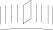
\includegraphics[height=3em]{generic-freeness}

      \hil{in commutative algebra} \\
      new reduction techniques \\
      constructive proofs
    \end{column}

    \hspace*{-1em}

    \begin{column}{0.56\textwidth}
      \centering
      \includegraphics[height=3em]{calabi-yau}

      \hil{in algebraic geometry} \\
      simpler and more conceptual proofs \\
      \mbox{reducing relative to absolute} \\
      synthetic algebraic geometry
    \end{column}
  \end{columns}

  \bigskip

  \begin{columns}
    \hspace*{-1.5em}

    \begin{column}{0.56\textwidth}
      \centering
      \includegraphics[height=3em]{filmat}

      \hil{in philosophy of math} \\
      historical contingency \\
      platonism \\
      pluralism \\
      relativism
    \end{column}

    \hspace*{-1em}

    \begin{column}{0.56\textwidth}
      \centering
      \includegraphics[height=3em]{torus-rainbow}

      \hil{in further fields} \\
      synthetic measure theory \\
      synthetic computability theory \\
      synthetic homotopy theory (HoTT) \\
      Bohr topos for quantum mechanics
    \end{column}
  \end{columns}
\end{frame}

\begin{frame}{The little Zariski topos of a ring}
  Let~$A$ be a reduced commutative ring ($x^n = 0 \Rightarrow x = 0$).

  The \hil{little Zariski topos} of~$A$ is equivalently
  \vspace*{-0.5em}
  \begin{itemize}
    \item the topos of sheaves over~$\Spec(A)$,
    \item the classifying topos of local localizations of~$A$ or
    \item the classifying topos of prime filters of~$A$
  \end{itemize}
  \vspace*{-0.5em}
  and contains a \hil{mirror image} of~$A$: $A^\sim$.

  \vspace*{-1.5em}
  \small

  \begin{columns}
    \begin{column}{0.5\textwidth}
      \begin{varblock}{\textwidth}{}
        \justifying
        Assuming the Boolean prime ideal theorem, a first-order
        formula ``$\forall \ldots \forall\_ (\cdots \Longrightarrow \cdots\!\,)$'',
        where the two subformulas may not contain~``$\Rightarrow$'' and~``$\forall$'',
        holds for~$A^\sim$ iff it holds for all stalks~$A_\ppp$.
      \end{varblock}
    \end{column}

    \begin{column}{0.5\textwidth}
      \begin{varblock}{\textwidth}{}
        $A^\sim$ inherits any property of~$A$ which is
        \hil{localization-stable}.
      \end{varblock}

      \vspace*{-1.7em}

      \setbeamercolor{block body}{bg=red!30}
      \setbeamercolor{structure}{fg=purple}
      \begin{varblock}{\textwidth}{}
        $A^\sim$ is a \hil{local ring} and a \hil{field}.

        $A^\sim$ has \hil{$\boldsymbol{\neg\neg}$-stable equality}.

        \mbox{$A^\sim$ is \hil{anonymously Noetherian}.}\\[-1.2em]
      \end{varblock}
    \end{column}
  \end{columns}

  \visible<2>{\begin{tikzpicture}[overlay]
    \draw[fill=white, draw=white, opacity=0.95] (-1,0) rectangle (\paperwidth,7.4);
    \node[anchor=south west,inner sep=0] (image) at (0,0.8) {\vbox{
      \centering
      \includegraphics[width=0.9\textwidth]{tierney-on-the-spectrum-of-a-ringed-topos} \\
      \footnotesize
      Miles Tierney. On the spectrum of a ringed topos. 1976.
    }};
  \end{tikzpicture}}
\end{frame}

\begin{frame}{Applications in commutative algebra}
  Let~$A$ be a reduced commutative ring ($x^n = 0 \Rightarrow x = 0$). \\
  Let~$A^\sim$ be its mirror image in the little Zariski topos.

  \small
  \begin{columns}[t]
    \begin{column}[t]{0.46\textwidth}
      \centering

      \scalebox{0.8}{$\begin{pmatrix}
        \cdot & \cdot & \cdot & \cdot & \cdot \\
        \cdot & \cdot & \cdot & \cdot & \cdot \\
        \cdot & \cdot & \cdot & \cdot & \cdot
      \end{pmatrix}$}
      \vspace*{-1em}

      \begin{varblock}{\textwidth}{A baby application}
        \justifying
        Let~$M$ be an injective matrix over~$A$ with more columns than rows.
        Then~$1 = 0$ in~$A$.
      \end{varblock}

      \justifying
      \textbf{Proof.} $M$ is also injective as a matrix over~$A^\sim$.
      Since~$A^\sim$ is a field, trivially~$1 = 0$ in~$A^\sim$.
      This means~$1 = 0$ in~$A$.
    \end{column}

    \begin{column}[t]{0.57\textwidth}
      \centering

      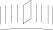
\includegraphics[height=3em]{generic-freeness}
      \vspace*{-1em}

      \begin{varblock}{\textwidth}{Generic freeness\phantom{p}}
        \justifying
        Let~$M$ be a finitely generated~$A$-module.
        If~$f = 0$ is the only element of~$A$ such that~$M[f^{-1}]$ is a
        free~$A[f^{-1}]$-module, then~$1 = 0$ in~$A$.
      \end{varblock}
      \vspace*{-0.5em}

      \raggedright
      \textbf{Proof.} The claim is the translation of the statement~``$M^\sim$
      is \hil{not not} free''. Since~$A^\sim$ is a field, this is trivial.
    \end{column}
  \end{columns}
\end{frame}

\begin{frame}{The Kripke--Joyal semantics for the little Zariski topos}
  Recall~$A[f^{-1}] = \bigl\{ \frac{u}{f^n} \,|\, u \in A, n \in \NN \bigr\}$.

  \begin{itemize}
    \item $\Sh(\Spec(A)) \models \text{``For all~$x \in A^\sim$, \ldots''}$

          Meaning: For all~$f \in A$ and all~$x \in A[f^{-1}]$, \ldots
          \medskip

    \item $\Sh(\Spec(A)) \models \text{``There is~$x \in A^\sim$ such that \ldots''}$

          \mbox{Meaning: There is a partition of unity,~$1 = f_1 + \cdots + f_n \in A$,}
          such that for each~$i$, there exists~$x_i \in A[f_i^{-1}]$
          with~\ldots
          \medskip

    \item $\Sh(\Spec(A)) \models \text{``$\varphi$ implies $\psi$''}$

          Meaning: For all~$f \in A$, if~$\varphi$ on stage~$f$, then~$\psi$ on
          stage~$f$.
  \end{itemize}
\end{frame}

\begin{frame}{Applications in algebraic geometry}
  \vspace*{-1.5em}
  \begin{varblock}{0.9\textwidth}{}
    \justifying
    Understand notions of algebraic geometry over a scheme~$X$ as
    notions of algebra internal to~$\Sh(X)$.
  \end{varblock}

  \small\centering
  \scalebox{0.83}{\begin{tabular}{ll}
    \toprule
    externally & internally to $\Sh(X)$ \\
    \midrule
    sheaf of sets & set \\
    %sheaf of rings & ring \\
    sheaf of modules & module \\
    sheaf of finite type & finitely generated module \\
    % finite locally free sheaf & finite free module \\
    % coherent sheaf & coherent module \\
    tensor product of sheaves & tensor product of modules \\
    % sheaf of Kähler differentials & module of Kähler differentials \\
    sheaf of rational functions & total quotient ring of~$\O_X$ \\
    dimension of $X$ & Krull dimension of~$\O_X$ \\
    spectrum of a sheaf of~$\O_X$-algebras & ordinary spectrum [with a twist] \\
    higher direct images & sheaf cohomology \\
    \bottomrule
  \end{tabular}}

  \begin{columns}[c]
    \begin{column}{0.43\textwidth}
      \begin{exampleblock}{}
        \justifying
        Let~$0 \to M' \to M \to M'' \to 0$ be a short exact sequence of
        modules. If~$M'$ and~$M''$ are finitely generated, so is~$M$.
      \end{exampleblock}
    \end{column}

    \scalebox{3}{$\Rightarrow$}
    \hspace*{0.5em}

    \begin{column}{0.47\textwidth}
      \begin{exampleblock}{}
        \justifying
        Let $0 \to \F' \to \F \to \F'' \to 0$ be a short exact sequence
        of sheaves of~$\O_X$-modules. If~$\F'$ and~$\F''$ are of finite type,
        so is~$\F$.
      \end{exampleblock}
    \end{column}
  \end{columns}
\end{frame}

\begin{frame}{Synthetic algebraic geometry}
  Usual approach to algebraic geometry: \hil{layer schemes above ordinary set theory}
  using either
  \begin{itemize}
    \item locally ringed spaces
    \small
    \begin{multline*}
      \text{set of prime ideals of~$\ZZ[X,Y,Z]/(X^n+Y^n-Z^n)$} + {} \\
      \text{Zariski topology} + \text{structure sheaf}
    \end{multline*}
    \normalsize
    \item or Grothendieck's functor-of-points account, where a scheme is a functor~$\mathrm{Ring} \to \mathrm{Set}$.
    \small\[ A \longmapsto \{ (x,y,z) \in A^3 \,|\, x^n+y^n-z^n=0 \} \]
  \end{itemize}
  \bigskip
  \pause

  \hil{Synthetic approach:} model schemes \hil{directly as sets} in a certain
  nonclassical set theory, the internal universe of the \mbox{\hil{big Zariski
  topos}} of a base scheme.
  \small
  \[ \{ (x,y,z) \? (\affl)^3 \,|\, x^n+y^n-z^n=0 \} \]
\end{frame}

\begin{frame}{The big Zariski topos}
  The \hil{big Zariski topos} $\Zar(S)$ of a scheme~$S$ is equivalently
  \begin{enumerate}
    \item the topos of sheaves over~$\Aff/S$,
    \item the classifying topos of local rings over~$S$ or
    \item the classifying~$\Sh(S)$-topos of local~$\O_S$-algebras which are local
    over~$\O_S$.
  \end{enumerate}

  \begin{itemize}
    \item For an~$S$-scheme~$X$, its functor of points $\ull{X} =
    \Hom_S(\cdot,X)$ is an object of~$\Zar(S)$. It feels like \hil{the set of
    points} of~$X$.
    \item Internally, $\affl$ (given by $\affl(T) = \O_T(T)$)
    looks like a field
    %\[ \Zar(S) \models \forall x\?\affl\_ x \neq 0 \Longrightarrow \text{$x$ invertible} \]
    and is \hil{synthetically quasicoherent}: For any finitely
    presented~$\affl$-algebra~$B$, the canonical map is bijective.
    \[ B \longrightarrow (\affl)^{\Hom_\affl(B,\affl)},\ f \longmapsto (\varphi \mapsto \varphi(f)) \]
    \item \ \\[-1.2em]\mbox{$\ull{\mathbb{P}}^n = \llbracket \{ (x_0,\ldots,x_n) : (\affl)^{n+1} \,|\,
    x_0 \neq 0 \vee \cdots \vee x_n \neq 0 \}/(\affl)^\times \rrbracket$}
  \end{itemize}
\end{frame}


\section{Vision}

\begin{frame}{Vision for the future}
  \begin{columns}
    \small
    \begin{column}{0.35\textwidth}
      \centering
      \bigheart
      \par

      constructive algebra \\
      conceptual proofs \\
      proof assistants
    \end{column}

    \begin{column}{0.47\textwidth}
      \centering
      \bigheart
      \par

      constructive algebraic geometry \\
      synthetic algebraic geometry \\
      intersection theory \\
      derived categories
    \end{column}

    \begin{column}{0.25\textwidth}
      \centering
      \bigheart
      \par

      quasicoherence \\
      nongeometric mysteries \\
      further fields
    \end{column}
  \end{columns}

  \vfill

  \centering
  \href{https://www.oliviacaramello.com/Papers/Papers.htm}{\includegraphics[height=0.45\textheight]{olivia-tst}}
  \href{http://math.andrej.com/2014/03/04/intuitionistic-mathematics-and-realizability-in-the-physical-world/}{\includegraphics[height=0.45\textheight]{zenil-computable-universe}}
  \href{https://pizzaseminar.speicherleck.de/skript2/zariski-topos-klein.pdf}{\includegraphics[height=0.45\textheight]{fun-with-the-zariski-topos}}
  \href{https://rawgit.com/iblech/internal-methods/master/notes.pdf}{\includegraphics[height=0.45\textheight]{phd-cover}}
\end{frame}

\addtocounter{framenumber}{-1}

\end{document}
